\documentclass[tikz,border=4pt]{standalone}
\usepackage{amssymb}
\usepackage{tikz}
\usetikzlibrary{positioning,shapes.geometric,arrows.meta,fit,calc,backgrounds}

% --- BNN palette ---
\definecolor{ctrlFill}{HTML}{dae8fc}
\definecolor{ctrlStroke}{HTML}{6c8ebf}
\definecolor{memFill}{HTML}{ffe6cc}
\definecolor{memStroke}{HTML}{d79b00}
\definecolor{calcFill}{HTML}{cce5ff}
\definecolor{calcStroke}{HTML}{4a86e8}
\definecolor{dataFill}{HTML}{d5e8d4}
\definecolor{dataStroke}{HTML}{82b366}
\definecolor{pkrnCol}{HTML}{c44b3a}
\definecolor{hubFill}{HTML}{f8cecc}
\definecolor{hubStroke}{HTML}{b85450}
\definecolor{newStroke}{HTML}{b85450}

\begin{document}
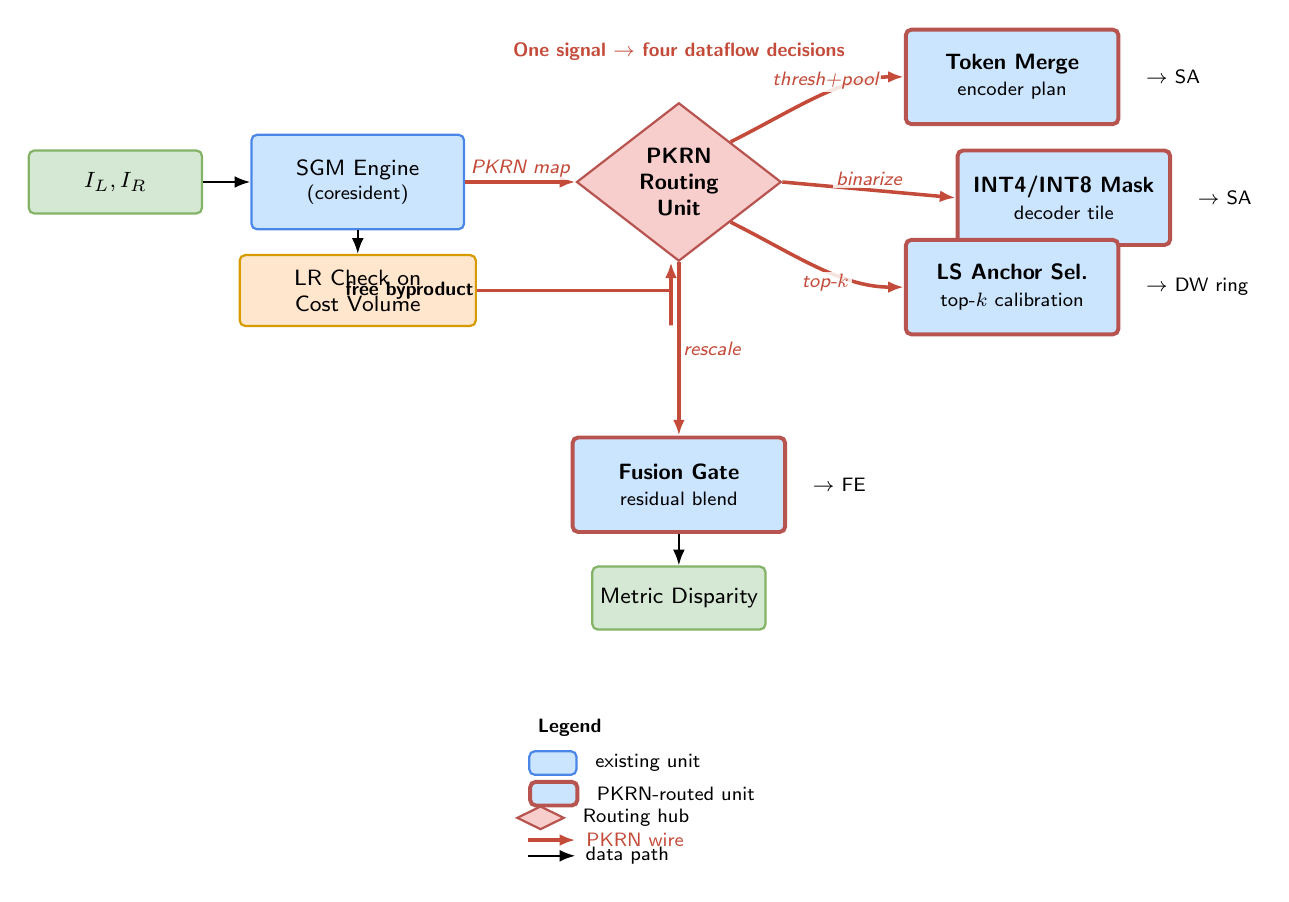
\begin{tikzpicture}[
  font=\footnotesize\sffamily,
  ctrl/.style={draw=ctrlStroke, fill=ctrlFill, rounded corners=2pt, thick,
               minimum width=24mm, minimum height=9mm, align=center, inner sep=2pt},
  calc/.style={draw=calcStroke, fill=calcFill, rounded corners=2pt, thick,
               minimum width=27mm, minimum height=12mm, align=center, inner sep=2pt},
  newcalc/.style={draw=newStroke, fill=calcFill, rounded corners=2pt, line width=0.5mm,
                  minimum width=27mm, minimum height=12mm, align=center, inner sep=2pt},
  mem/.style={draw=memStroke, fill=memFill, rounded corners=2pt, thick,
              minimum width=27mm, minimum height=9mm, align=center, inner sep=2pt},
  data/.style={draw=dataStroke, fill=dataFill, rounded corners=2pt, thick,
               minimum width=22mm, minimum height=8mm, align=center, inner sep=2pt},
  hub/.style={draw=hubStroke, fill=hubFill, diamond, thick,
              minimum width=26mm, minimum height=18mm, align=center, inner sep=1pt,
              font=\footnotesize\sffamily\bfseries},
  arr/.style={-{Latex[length=2mm]}, thick},
  pkrnarr/.style={-{Latex[length=2mm]}, draw=pkrnCol, line width=0.45mm},
  xflbl/.style={font=\scriptsize\sffamily\itshape, text=pkrnCol, inner sep=1pt, fill=white, fill opacity=0.85, text opacity=1}
]

% ============ LEFT: UPSTREAM FREE SGM ============
\node[data] (img) at (0,0) {$I_L,I_R$};
\node[calc, right=6mm of img] (sgm) {SGM Engine\\[-1pt]\scriptsize(coresident)};
\node[mem, below=3mm of sgm, minimum width=30mm] (lrc) {LR Check on\\Cost Volume};
\node[xflbl, left=0mm of lrc.east, anchor=east, text=black, fill=none] {\textbf{free byproduct}};

\draw[arr] (img) -- (sgm);
\draw[arr] (sgm.south) -- (lrc.north);

% ============ HUB ============
\node[hub, right=14mm of sgm] (hub) {PKRN\\Routing\\Unit};
\draw[pkrnarr] (lrc.east) -| ($(hub.south)+(-1mm,-8mm)$) -- ($(hub.south)+(-1mm,0)$);
\draw[pkrnarr] (sgm.east) -- node[xflbl, above]{PKRN map}  (hub.west);

% ============ FOUR SPOKES (2x2 grid of consumer units) ============
\node[newcalc, above right=2mm and 22mm of hub] (merge) {\textbf{Token Merge}\\\scriptsize encoder plan};
\node[newcalc, right=22mm of hub, yshift=-2mm] (prec)   {\textbf{INT4/INT8 Mask}\\\scriptsize decoder tile};
\node[newcalc, below right=2mm and 22mm of hub] (anch)  {\textbf{LS Anchor Sel.}\\\scriptsize top-$k$ calibration};
\node[newcalc, below=22mm of hub]               (gate)  {\textbf{Fusion Gate}\\\scriptsize residual blend};

% fan-out arrows with module-local transform labels
\draw[pkrnarr] (hub.north east) .. controls +(8mm,4mm) and +(-8mm,0mm) .. (merge.west)
  node[pos=0.55, xflbl, above] {thresh+pool};
\draw[pkrnarr] (hub.east) -- (prec.west)
  node[pos=0.5, xflbl, above] {binarize};
\draw[pkrnarr] (hub.south east) .. controls +(8mm,-4mm) and +(-8mm,0mm) .. (anch.west)
  node[pos=0.55, xflbl, below] {top-$k$};
\draw[pkrnarr] (hub.south) -- (gate.north)
  node[pos=0.5, xflbl, right] {rescale};

% consumer destinations (tiny tag on right)
\node[font=\scriptsize\sffamily, right=2mm of merge] {$\to$ SA};
\node[font=\scriptsize\sffamily, right=2mm of prec]  {$\to$ SA};
\node[font=\scriptsize\sffamily, right=2mm of anch]  {$\to$ DW ring};
\node[font=\scriptsize\sffamily, right=2mm of gate]  {$\to$ FE};

% ============ OUTPUT ============
\node[data, below=4mm of gate] (out) {Metric Disparity};
\draw[arr] (gate.south) -- (out.north);

% ============ TITLE BANNER (below hub, above nothing) ============
\node[font=\scriptsize\sffamily\bfseries, text=pkrnCol, above=4mm of hub]
  {One signal $\to$ four dataflow decisions};

% ============ LEGEND ============
\begin{scope}[shift={($(out.south west)+(-8mm,-10mm)$)}]
  \node[anchor=north west, font=\scriptsize\sffamily\bfseries] (lh) at (0,0) {Legend};
  \node[calc, minimum width=6mm, minimum height=3mm, below=0.5mm of lh.south west, anchor=north west, inner sep=1pt] (L1) {};
  \node[right=1mm of L1, font=\scriptsize\sffamily] {existing unit};
  \node[newcalc, minimum width=6mm, minimum height=3mm, below=0.5mm of L1.south west, anchor=north west, inner sep=1pt] (L2) {};
  \node[right=1mm of L2, font=\scriptsize\sffamily] {PKRN-routed unit};
  \node[hub, minimum width=6mm, minimum height=3mm, below=0.5mm of L2.south west, anchor=north west, inner sep=1pt] (L3) {};
  \node[right=1mm of L3, font=\scriptsize\sffamily] {Routing hub};
  \draw[pkrnarr] ([yshift=-2mm]L3.south west) -- ++(6mm,0)
    node[right, font=\scriptsize\sffamily, text=pkrnCol] {PKRN wire};
  \draw[arr] ([yshift=-4mm]L3.south west) -- ++(6mm,0)
    node[right, font=\scriptsize\sffamily] {data path};
\end{scope}

\end{tikzpicture}
\end{document}
